\subsubsection{Analysis of Airfoil}

First we analyse the Airfoil application from the OP2 library --- this is the
most well understood and thoroughly studied example, therefore we go into more
detail here --- for later kernels and applications we then identify key
differences.

Table \ref{tab:airfoil_counters_glob} show the effect of various optimisations on the Airfoil application (\textbf{res\_calc}
kernel).

\emph{Global colouring}: The SoA layout, as mentioned in Section \ref{aos-to-soa}, improves on the
performance, since the threads in a warp access data addresses that are near
each other. This can also be seen in the number of global memory read
transactions as it is roughly $87\%$ of that with AoS layout. This is even
further improved by the GPS renumbering, which places data points that are accessed in
consecutive threads close to each other ($19\%$ reduction in global read
transactions compared to AoS). The partition based reordering is primarily intended for the hierarchical
colouring; it groups threads that access the same data together, while the
global colouring puts them into different kernel launches, eliminating any
chance for spatial reuse, therefore reducing performance.

\begin{table}[Htbp]
  \centering
  \resizebox{\columnwidth}{!}{
    % TODO either fill in the missing data or undo the whole unification of the
    % two tables
  \begin{tabular}{|R{3cm}|c|c|c|c||c|c|c|c||c|}
    \hline
                       Colouring  & \multicolumn{4}{c||}{Global} & \multicolumn{4}{c||}{Hierarchical} & \begin{tabular}{@{}c@{}}Original \\ Hierarchical\end{tabular}\\
                       \hline
                      Reordering  & \multicolumn{2}{c|}{none} & GPS & partition & \multicolumn{2}{c|}{none} & \multicolumn{2}{c||}{partition} & none\\
                      \hline
               Data layout &    AOS      &   SOA     &     SOA      &    SOA & AOS      &   SOA     &     AOS      &    SOA & SOA\\
               \hline
                         Bandwidth (GB/s)&  $71$ & $94$ &  $105$&  $67$&    $ 212$ &   $ 227$ &      $ 270$ &   $ 225$ & $ 233$\\ % 229 with the figure generated thing
                         \hline
                         Runtime (ms) & $6.12$ & $4.65$ & $4.15$ & $6.64$ & $2.07$ & $2.03$ & $1.92$ & $1.83$ & $1.91$\\
                      \hline
                Achieved Occupancy&  $0.63$ &  $0.45$ &      $0.45$&            $0.45$&    $0.44$ &   $0.52$ &      $0.59$ &   $0.42$ & $0.42$\\
                      \hline
    Global Memory Read Transactions&  \num{52424}k & \num{45781}k &      \num{41246}k&            \num{66775}k&    \num{21142}k & \num{21192}k &      \num{13964}k &   \num{14406}k&  \num{21866}k\\
                      \hline
    Global Memory Write Transactions&  \num{14007}k &  \num{14737}k &      \num{13773}k&            \num{20733}k&     \num{5807}k &   \num{57883}k &       \num{3397}k &    \num{3669}k&  \num{6384}k\\
                      \hline
                 Number of (Block) Colours&  $5$&  $5$ &      $5$ &            $7$&    $       4$ &   $       5$ &      $       8$ &   $       8$ &   $       5$\\
                      \hline
                       Number of Thread Colours&-&-&-&-&    $       3$ &   $       3$ &      $       4$ &   $       4$ &   $       3$\\
                      \hline
                                   Reuse Factor&-&-&-&-&    $       2$ &   $       2$ &      $     3.6$ &   $     3.6$ &   $       2$\\
                      \hline
          Issue Stall Reasons (Synchronization)&-&-&-&-&    $  11\%$ &   $   9\%$ &      $  14\%$ &   $  14\%$ &   $  14\%$\\
                      \hline
             Issue Stall Reasons (Data Request)&-&-&-&-&    $  69\%$ &   $  68\%$ &      $  61\%$ &   $  63\%$ &   $  55\%$\\
             \hline
             Block Size &\multicolumn{8}{c||}{$480$} &   $128$\\
             \hline
  \end{tabular}
  }
  \caption{Collected performance metrics of the global and hierarchical
  colouring implementation of the \textbf{res\_calc} kernel.}
  \label{tab:airfoil_counters_glob}
\end{table}


%%%%%%%%%%%%%%%%%%%%%%%%%%%%%%%%%%%%%%%%%%%%%%%%%%%%%%%%%%%%
% airfoil hierarchical

\emph{Hierarchical colouring:}  The key goal of this strategy is to better exploit data reuse by using the
shared memory; the results of which show immediately in the number of global
transactions as well, shown in Table \ref{tab:airfoil_counters_glob}: at block size $480$, there is roughly $60\%$ decrease in
global read and write transactions, leading to three times the performance. Throughput for different block sizes is shown in Figure \ref{fig:airfoil_bw-vs-bs_hier_large}.

These also show that the reordering using partitioning is indeed effective. With
a block size of 448, data reuse increased from $2$ with the reference version,
to $3.6$, leading to the $19\%$ performance gain over the version without
reordering (AoS layout). This is also consistent with the number of global
transactions: there is a $35\%$ decrease in the number of reads and $41\%$
decrease in the number of writes, and a decrease in the percentage of stalls
occurring because of data requests: $61\%$ with partitioning, $68\%$ without.

With the increased reuse, the number of thread colours is also larger ($4$
versus $2.2$) and this leads to more synchronisation: with reordering, $14\%$
of the stalls were caused by synchronisation, up from $9\%$.

This is further illustrated by Figure \ref{fig:airfoil_speedup_large} that shows
the relative speedup compared to the original OP2 version. In this case, the
original version also used the shared memory approach, so the performance gain
is caused by the reordering. In the original version $56\%$ of the total time is spent
in \textbf{res\_calc}, therefore the achieved $1.2\times$ speedup on \textbf{res\_calc}
causes about $1.1\times$ speedup on the whole application. The useful bandwidth in case
of the best version of \textbf{res\_calc} reached $55\%$ of the peak stream bandwidth of
the P100 GPU.

% Figure \ref{fig:airfoil_bw-vs-bs_hier_large} shows performance variations at different block sizes with the hierarchical colouring approach. This kernel uses more registers ($52$ (SoA) and $48$ (AoS)) compared to global
% colouring ($48$ and $40$), which leads to larger variations in occupancy and
% performance as the block size changes; for example, between block sizes $480$
% and $448$ ($44\%$ versus $51\%$).

% airfoil profiler counters {{{ %
% table hier {{{2 %
% Block size: 480                                                                                                            448
% Hier
%                                                      NR/AOS     NR/SOA      GPS/AOS     GPS/SOA   METIS/AOS   METIS/SOA     NR/AOS      NR/SOA     GPS/AOS      GPS/SOA  METIS/AOS    METIS/SOA
%                              Achieved Occupancy    0.443160    0.429204    0.439582    0.428747    0.444403    0.425626    0.515455    0.363607    0.589185    0.401288    0.586993    0.419531
%     Shared Memory Load Transactions Per Request    3.188424    2.555526    2.694831    2.040550    4.110473    3.708974    3.409922    2.743898    2.714740    2.033035    4.086514    3.704884
%    Shared Memory Store Transactions Per Request    2.584290    2.584290    2.064633    2.064633    3.735147    3.735147    2.781154    2.781154    2.063529    2.063529    3.699993    3.699993
%                   Device Memory Read Throughput  301.18GB/s  311.13GB/s  302.61GB/s  307.53GB/s  210.01GB/s  230.71GB/s  327.64GB/s  302.84GB/s  329.21GB/s  303.88GB/s  255.14GB/s  216.66GB/s
%                  Device Memory Write Throughput  82.725GB/s  85.869GB/s  83.002GB/s  85.152GB/s  51.859GB/s  58.425GB/s  89.488GB/s  83.716GB/s  89.591GB/s  84.246GB/s  62.061GB/s  55.181GB/s
%                        Shared Memory Efficiency      63.34%      70.80%      79.52%      91.75%      44.41%      46.56%      62.16%      69.36%      82.28%      95.47%      43.88%      46.11%
%                       Warp Execution Efficiency      98.31%      98.21%      98.82%      98.64%      98.30%      98.11%      98.91%      98.70%      99.32%      99.05%      98.07%      98.30%
%                            L2 Read Transactions     7420757     5778724     6023832     4857165     2316268     1988909     5474855     4608456     5744884     4841211     2419295     1974515
%                    L2 Read Transactions (total)    29683028    23114896    30119160    24285825    18530144    15911272    27374275    23042280    28724420    24206055    19354360    15796120
%                           L2 Write Transactions     1442624     1595887     1154859     1279265      403567      477997     1154275     1281658     1155450     1277893      405007      480049
%                   L2 Write Transactions (total)     5770496     6383548     5774295     6396325     3228536     3823976     5771375     6408290     5777250     6389465     3240056     3840392
%            Global Load Transactions Per Request   14.812981   10.226367   14.895732   10.832033   15.735381   11.959669   14.936378   10.325527   14.886971   10.819459   15.739796   12.034410
%           Global Store Transactions Per Request   15.519316    8.315796   15.556413    8.347770   15.681818    8.835123   15.485325    8.342052   15.525290    8.299908   15.649229    9.232377
%                 Device Memory Read Transactions     5285507     5318626     4249079     4266665     1735615     1790665     4238592     4262383     4266830     4270567     1745529     1800764
%         Device Memory Read Transactions (total)    21142028    21274504    21245395    21333325    13884920    14325320    21192960    21311915    21334150    21352835    13964232    14406112
%                Device Memory Write Transactions     1451764     1467868     1165479     1181414      428595      453474     1157662     1178263     1161173     1183936      424586      458638
%        Device Memory Write Transactions (total)     5807056     5871472     5827395     5907070     3428760     3627792     5788310     5891315     5805865     5919680     3396688     3669104
%                      Unified Cache Transactions    11169643    11541464     8935482     9230798     5196985     5381043     8936518     9234659     8936606     9232591     5199650     5384917
%              Unified Cache Transactions (total)    44678572    46165856    44677410    46153990    41575880    43048344    44682590    46173295    44683030    46162955    41597200    43079336
%           Issue Stall Reasons (Synchronization)      10.69%       9.97%       8.21%       7.76%      14.60%      13.93%       8.97%       9.23%       7.57%       7.64%      13.60%      14.45%
%              Issue Stall Reasons (Data Request)      69.40%      70.46%      71.08%      71.65%      61.87%      64.22%      68.02%      66.92%      71.29%      72.55%      60.83%      62.53%
%      Issue Stall Reasons (Execution Dependency)       7.88%       9.22%       7.83%       9.82%       9.38%      10.99%       8.46%       9.52%       8.41%       9.70%       8.93%      11.56%
%                                      Issued IPC    0.474839    0.561239    0.468044    0.547087    0.483891    0.597130    0.481460    0.520914    0.503466    0.537601    0.580322    0.560527
%                                     Issue Slots    14324106    16698536    11307496    13207634     6693306     7962453    11400009    13301504    11245197    13146824     6706368     7945731
%                             Issue Slots (total)    57296424    66794144    56537480    66038170    53546448    63699624    57000045    66507520    56225985    65734120    53650944    63565848
%                          Issue Slot Utilization      20.84%      24.74%      20.61%      24.18%      21.15%      26.48%      21.12%      22.96%      22.15%      23.75%      25.37%      24.87%
%                 Eligible Warps Per Active Cycle    0.580331    0.780844    0.575476    0.774725    0.593362    0.834286    0.581190    0.706083    0.616539    0.754858    0.722055    0.741442
%                               Branch Efficiency      99.71%      99.70%      99.70%      99.69%      99.70%     100.00%      99.69%      99.68%      99.68%      99.67%      99.67%     100.00%
%        Warp Non-Predicated Execution Efficiency      95.00%      95.36%      95.70%      95.96%      95.07%      95.57%      95.63%      95.88%      96.18%      96.35%      94.84%      95.75%
%                    FLOP Efficiency(Peak Single)       0.00%       0.00%       0.00%       0.00%       0.00%       0.00%       0.00%       0.00%       0.00%       0.00%       0.00%       0.00%
%                    FLOP Efficiency(Peak Double)       6.18%       6.34%       6.19%       6.27%       6.42%       6.84%       5.45%       5.00%       6.70%       6.18%       7.75%       6.39%
%                   L2 Throughput (Texture Reads)  425.94GB/s  338.07GB/s  431.15GB/s  350.67GB/s  280.17GB/s  255.97GB/s  423.17GB/s  327.57GB/s  444.88GB/s  343.27GB/s  353.48GB/s  237.36GB/s
%                                    Executed IPC    0.473607    0.559122    0.468013    0.547363    0.482661    0.596862    0.473772    0.519968    0.502728    0.537943    0.579599    0.560211
%                         Multiprocessor Activity      97.63%      98.48%      97.21%      98.01%      95.03%      95.96%      78.72%      79.35%      97.57%      97.86%      95.66%      95.31%
%                         Number of Block Colours           4           4           5           5           8           8           5           5           5           5           8           8
%                                    Reuse Factor           2           2           2           2         3.6         3.6           2           2           2           2         3.6         3.6
%                        Number of Thread Colours           3           3         2.2         2.2           4           4           3           3         2.2         2.2           4           4
%                                       Bandwidth     212GB/s     215GB/s     211GB/s     213GB/s     228GB/s     240GB/s     227GB/s     209GB/s     227GB/s     210GB/s     270GB/s     225GB/s
%                               Partitioning time                                                    57s                                                                      61s
% 2}}} %

% Global:
%                                                      NR/AOS      NR/SOA     GPS/AOS     GPS/SOA   METIS/AOS   METIS/SOA
%                              Achieved Occupancy    0.631237    0.452564    0.631344    0.452512    0.635776    0.453620
%     Shared Memory Load Transactions Per Request    0.000000    0.000000    0.000000    0.000000    0.000000    0.000000
%    Shared Memory Store Transactions Per Request    0.000000    0.000000    0.000000    0.000000    0.000000    0.000000
%                   Device Memory Read Throughput  248.98GB/s  288.34GB/s  248.96GB/s  291.34GB/s  232.15GB/s  292.22GB/s
%                  Device Memory Write Throughput  66.524GB/s  92.816GB/s  66.053GB/s  97.286GB/s  63.233GB/s  90.733GB/s
%                        Shared Memory Efficiency       0.00%       0.00%       0.00%       0.00%       0.00%       0.00%
%                       Warp Execution Efficiency     100.00%     100.00%     100.00%     100.00%     100.00%     100.00%
%                            L2 Read Transactions    14565452    16965768    14323192    15996232    11918764    13498242
%                    L2 Read Transactions (total)    72827260    84828840    71615960    79981160    83431348    94487694
%                           L2 Write Transactions     9766867     6753853     9636030     6429508     7291602     5659277
%                   L2 Write Transactions (total)    48834335    33769265    48180150    32147540    51041214    39614939
%            Global Load Transactions Per Request   23.716634   17.915511   23.325628   17.101681   24.002277   19.996529
%           Global Store Transactions Per Request   31.999555   23.452729   31.999404   21.522510   31.999733   27.328754
%                 Device Memory Read Transactions    10484810     9156247    10117322     8249230     8167543     9539239
%         Device Memory Read Transactions (total)    52424050    45781235    50586610    41246150    57172801    66774673
%                Device Memory Write Transactions     2801458     2947329     2684330     2754617     2224669     2961920
%        Device Memory Write Transactions (total)    14007290    14736645    13421650    13773085    15572683    20733440
%                      Unified Cache Transactions     8347940     8779730     8348009     8779803     5962864     6271288
%              Unified Cache Transactions (total)    41739700    43898650    41740045    43899015    41740048    43899016
%           Issue Stall Reasons (Synchronization)       0.00%       0.00%       0.00%       0.00%       0.00%       0.00%
%              Issue Stall Reasons (Data Request)      41.72%      85.01%      43.17%      87.06%      37.95%      85.24%
%      Issue Stall Reasons (Execution Dependency)       0.48%       6.75%       0.54%       5.36%       0.46%       6.65%
%                                      Issued IPC    0.078453    0.142348    0.087186    0.164855    0.068284    0.099497
%                                     Issue Slots     5763294     8064948     5763708     8064951     4118350     5762250
%                             Issue Slots (total)    28816470    40324740    28818540    40324655    28828450    40335750
%                          Issue Slot Utilization       3.47%       6.43%       3.85%       7.45%       3.02%       4.49%
%                 Eligible Warps Per Active Cycle    0.075685    0.155353    0.085263    0.184074    0.065787    0.108148
%                               Branch Efficiency     100.00%     100.00%     100.00%     100.00%     100.00%     100.00%
%        Warp Non-Predicated Execution Efficiency      99.45%      99.60%      99.45%      99.59%      99.45%      99.60%
%                    FLOP Efficiency(Peak Single)       0.00%       0.00%       0.00%       0.00%       0.00%       0.00%
%                    FLOP Efficiency(Peak Double)       1.98%       2.62%       2.18%       3.04%       1.69%       1.83%
%                   L2 Throughput (Texture Reads)  346.15GB/s  534.64GB/s  352.32GB/s  564.77GB/s  339.52GB/s  413.48GB/s
%                                    Executed IPC    0.078677    0.142596    0.087071    0.164932    0.068151    0.099503
%                         Multiprocessor Activity      98.05%      98.06%      97.76%      98.25%      96.59%      97.88%
%                         Number of Block Colours           5           5           5           5           7           7
%                                       Bandwidth      71GB/s      94GB/s      74GB/s     105GB/s      61GB/s      67GB/s
% At block size = 448, w/o sort-by-thread-col, BW (hier):
% METIS: AOS: 282GB/s, SOA: 267GB/s
% NR   : AOS: 227GB/s, SOA: 219GB/s (218/217 w/480bs)
% }}} airfoil profiler counters %

\begin{figure}[Htbp]
  \centering
  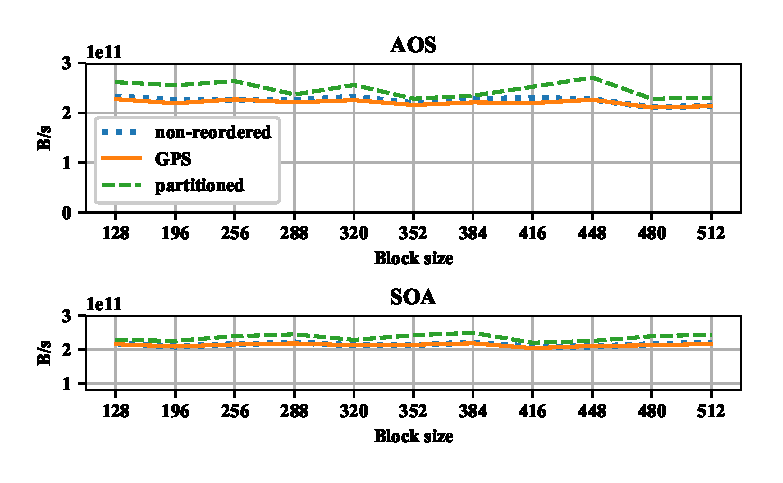
\includegraphics[width=9cm]{fig/airfoil_bw-vs-bs_hier_large.eps}
  \caption{\textbf{res\_calc} bandwidth on a dataset with $2880000$ cells with
  hierarchical colouring. Note that the y-axis doesn't start at the origin.}
  \label{fig:airfoil_bw-vs-bs_hier_large}
\end{figure}

\begin{figure}[Htbp]
  \centering
  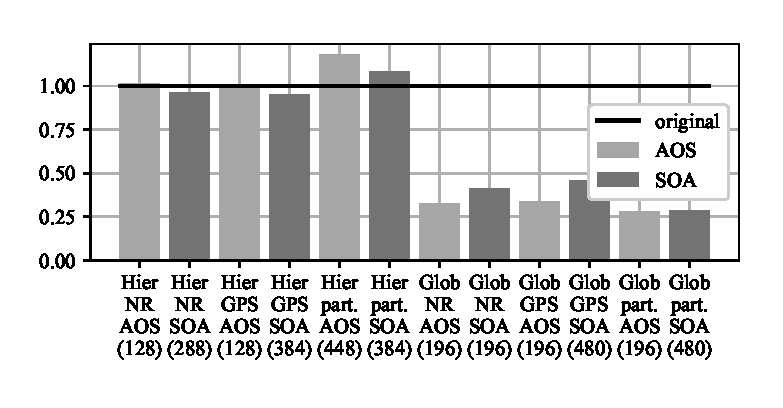
\includegraphics[width=9cm]{fig/airfoil_speedup_large.eps}
  \caption{\textbf{res\_calc} kernel speedup compared to the original code. Done
  on a dataset with $2800000$ cells. The block sizes are shown in parentheses,
  the reordering algorithms are: the original reordering (NR), GPS reordering
  and partitioning (part.)}
  \label{fig:airfoil_speedup_large}
\end{figure}

Although the number of block colours increased with reordering, it is only a
problem when the size of the dataset is so small that there are too few blocks for some colours to saturate the GPU.

When running on the newer Volta GPU architecture, the results look similar
(Figure \ref{fig:airfoil_bw-vs-bs_hier_large_volta}); the absolute value of the
bandwidths are (understandably) higher.

\begin{figure}[Htbp]
  \centering
  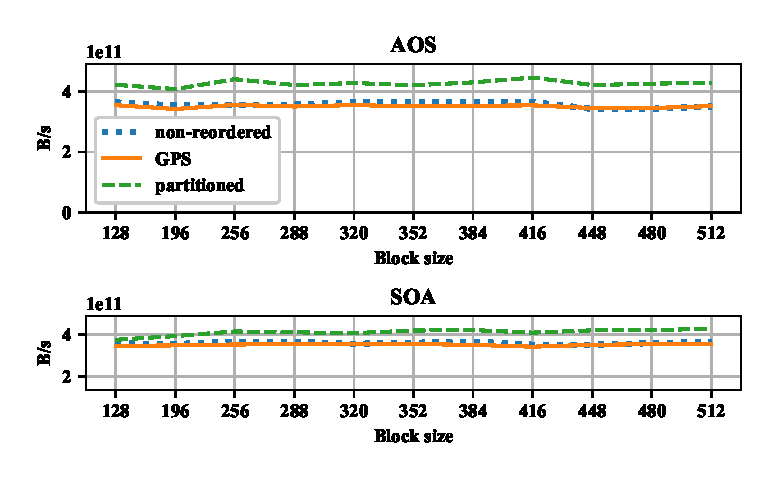
\includegraphics[width=9cm]{fig/airfoil_bw-vs-bs_hier_large_volta.eps}
  \caption{\textbf{res\_calc} bandwidth on a dataset with $2880000$ cells with
  hierarchical colouring, on Volta architecture. Note that the y-axis doesn't
  start at the origin.}
  \label{fig:airfoil_bw-vs-bs_hier_large_volta}
\end{figure}

On Volta, we achieved $1.28\times$ speedup in the kernel compared to the
original code with $446$ GB/s bandwidth ($60\%$ of the peak bandwidth). 
Since \textbf{res\_calc} takes around $54\%$ of the total run time in the
original code this speedup results in $1.14\times$ speedup on the
whole application.

\subsubsection{Analysis of Volna}

Measurements of the Volna application (\textbf{SpaceDiscretization} kernel)
with hierarchical colouring are shown in Figure \ref{fig:volna_bw-vs-bs_hier}  
and Table \ref{tab:volna_counters_hier}. The
reordering by partitioning again improves performance: it increases reuse from
$1.5$ to $2.8$ and decreases the number of global transactions by $18\%$ for
reads and $37\%$ for writes (Table \ref{tab:volna_counters_hier}). The larger
reduction in writes can be explained by the fact that the calculation does not
read the values of the indirect data from the previous iteration, only the
direct data.

Again, since the AoS version uses adjacent threads to load adjacent components
of data points, and also because one thread loads $4$ single precision values
into shared memory using the built-in vector type \lstinline!float4!, more data
can be transferred at the same time, thus there is a $2\%$ and $4\%$ reduction
in global memory transfers for reads and writes, respectively, leading to
increased performance ($292\,\text{GB/s}$ versus $268\,\text{GB/s}$).

Due to the low register counts ($28$--$32$) and the fact that volna uses float
(and int) datatypes compared to the doubles in Airfoil, the occupancy was quite
high (around $80\%$).  This explains the lack of dependence on the block size as
shown in the Figure \ref{fig:volna_bw-vs-bs_hier}.

Compared to Airfoil, the increase in the number of thread colours is less when
partitioning: from $3$ to $4$, hence, the synchronisation overhead is also less:
the percentage of stalls caused by synchronisation increases from $12\%$ to just
$15\%$. Of course, with high occupancy, the latency caused by synchronisation
can be better hidden by running warps from other blocks.

%shared memory usage:
% 7.7KB, 4.3 for metis

\begin{figure}[Htbp]
  \centering
  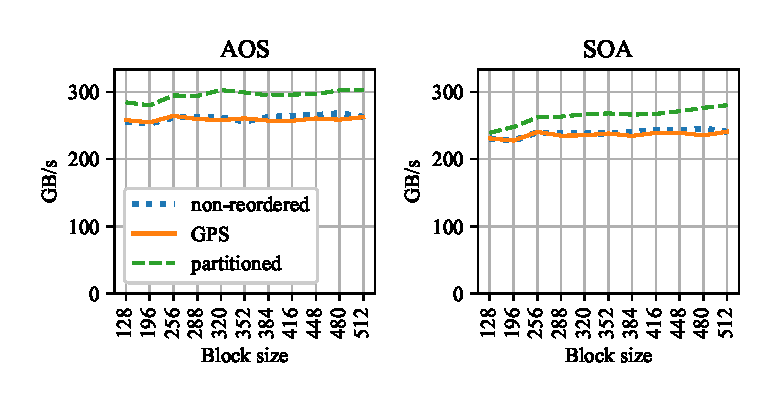
\includegraphics[width=9cm]{fig/volna_bw-vs-bs_hier.eps}
  \caption{\textbf{SpaceDiscretization} kernel bandwidth on a mesh with
  $3589735$ edges using hierarchical colouring. Note that the y-axis doesn't
  start at the origin.}
  \label{fig:volna_bw-vs-bs_hier}
\end{figure}

As can be seen from Figure \ref{fig:volna_speedup}, our implementation is $20\%$
faster than the original OP2 version. The $20\%$ performance gain in 
\textbf{SpaceDiscretization} results in $6\%$ increase regarding the whole 
application. The useful bandwidth also increased and reached $30\%$ of the peak 
stream bandwidth of the P100 GPU.

% volna counters {{{ %
% Block size: 448
% Hier:
%                                                      NR/AOS      NR/SOA     GPS/AOS     GPS/SOA   METIS/AOS   METIS/SOA
%                              Achieved Occupancy    0.819183    0.812192    0.815653    0.807516    0.796622    0.795811
%     Shared Memory Load Transactions Per Request    1.963101    1.963101    1.979188    1.979188    1.963848    1.963848
%    Shared Memory Store Transactions Per Request    1.961922    1.961922    1.978050    1.978050    1.973337    1.973337
%                   Device Memory Read Throughput  321.65GB/s  293.70GB/s  316.41GB/s  289.29GB/s  296.05GB/s  275.66GB/s
%                  Device Memory Write Throughput  86.010GB/s  80.508GB/s  85.125GB/s  80.088GB/s  60.913GB/s  59.338GB/s
%                        Shared Memory Efficiency      46.80%      46.80%      46.37%      46.37%      43.46%      43.46%
%                       Warp Execution Efficiency      98.21%      98.23%      98.19%      98.21%      96.98%      96.86%
%                            L2 Read Transactions     1843414     1858967     1536622     1551111      856125      871223
%                    L2 Read Transactions (total)     9217070     9294835     9219732     9306666     7705125     7841007
%                           L2 Write Transactions      495141      606426      413020      508079      150962      212536
%                   L2 Write Transactions (total)     2475705     3032130     2478120     3048474    13358658     1912814
%            Global Load Transactions Per Request    7.640348    7.339438    7.636162    7.336397    7.902319    7.678309
%           Global Store Transactions Per Request   16.172904    4.952004   16.187515    4.978461   15.811365    5.565519
%                 Device Memory Read Transactions     1822932     1833121     1519970     1529759      832512      846379
%         Device Memory Read Transactions (total)     9114660     9165605     9119820     9178554     7492608     7617411
%                Device Memory Write Transactions      487468      502498      408925      423507      171297      182190
%        Device Memory Write Transactions (total)     2437340     2512490     2453550     2541042     1541673     1639710
%                      Unified Cache Transactions     3654877     3744600     3045707     3120472     1881172     1917606
%              Unified Cache Transactions (total)    18274385    18274242    18274242    18722832    16930548    17258454
%           Issue Stall Reasons (Synchronization)      11.57%      11.72%      11.49%      11.60%      15.19%      14.60%
%              Issue Stall Reasons (Data Request)      50.79%      50.42%      50.14%      49.64%      45.80%      45.87%
%      Issue Stall Reasons (Execution Dependency)      16.93%      15.15%      17.00%      15.21%      16.41%      15.37%
%                                    Executed IPC    0.637022    0.630574    0.631593    0.625840    0.684925    0.661694
%                                      Issued IPC    0.638148    0.634302    0.633373    0.625643    0.686123    0.664217
%                                     Issue Slots     5963094     6515259     4972874     5433348     3101645     3319288
%                             Issue Slots (total)    29815470    32576295    29837244    32600088    27914805    29873592
%                          Issue Slot Utilization      27.35%      27.14%      27.15%      26.77%      29.39%      28.58%
%                         Multiprocessor Activity      95.44%      95.46%      93.98%      94.84%      92.02%      92.91%
%                 Eligible Warps Per Active Cycle    0.842456    0.842146    0.831790    0.828826    0.906572    0.878926
%                               Branch Efficiency      99.70%      99.70%      99.70%      99.70%     100.00%     100.00%
%        Warp Non-Predicated Execution Efficiency      94.27%      94.33%      94.25%      94.31%      92.74%      92.57%
%                    FLOP Efficiency(Peak Single)       1.64%       1.48%       1.60%       1.46%       1.68%       1.54%
%                    FLOP Efficiency(Peak Double)       0.00%       0.00%       0.00%       0.00%       0.00%       0.00%
%                   L2 Throughput (Texture Reads)  325.17GB/s  297.85GB/s  319.74GB/s  293.18GB/s  304.26GB/s  283.61GB/s
%                         Number of Block Colours           5           5           6           6           9           9
%                                    Reuse factor         1.5         1.5         1.5         1.5         2.8         2.8
%                       Average cache lines/block         300         307         300         308         165         184
%                        Number of Thread Colours           3           3           3           3           4           4
%                                       Bandwidth     265GB/s     241GB/s     260GB/s     238GB/s     292GB/s     268GB/s


% Glob:
%                                                   NR/AOS         NR/SOA     GPS/AOS     GPS/SOA   METIS/AOS   METIS/SOA
%                              Achieved Occupancy    0.766773    0.803794    0.769389    0.803205    0.766715    0.804845
%     Shared Memory Load Transactions Per Request    0.000000    0.000000    0.000000    0.000000    0.000000    0.000000
%    Shared Memory Store Transactions Per Request    0.000000    0.000000    0.000000    0.000000    0.000000    0.000000
%                   Device Memory Read Throughput  137.98GB/s  175.58GB/s  137.87GB/s  175.54GB/s  162.95GB/s  198.48GB/s
%                  Device Memory Write Throughput  66.312GB/s  92.108GB/s  66.360GB/s  92.292GB/s  76.224GB/s  100.73GB/s
%                        Shared Memory Efficiency       0.00%       0.00%       0.00%       0.00%       0.00%       0.00%
%                       Warp Execution Efficiency     100.00%     100.00%     100.00%     100.00%     100.00%     100.00%
%                            L2 Read Transactions     3874510     5586520     3886221     5599572     3230910     4083889
%                    L2 Read Transactions (total)    19372550    27932600    19431105    27997860    16154550    20419445
%                           L2 Write Transactions     5991159     4334428     6009907     4336008     5829332     3838742
%                   L2 Write Transactions (total)    29955795    21672140    30049535    21680040    29146660    19193710
%            Global Load Transactions Per Request   15.882479   13.241723   15.911647   13.244798   15.415391   12.327450
%           Global Store Transactions Per Request   31.580901   24.143615   31.673654   24.151083   30.845106   21.377642
%                 Device Memory Read Transactions     2790833     2409306     2793623     2410408     2653476     2414430
%         Device Memory Read Transactions (total)    13954165    12046530    13968115    12052040    13267380    12072150
%                Device Memory Write Transactions     1341294     1263924     1344665     1267340     1241239     1225405
%        Device Memory Write Transactions (total)     6706470     6319620     6723325     6336700     6206195     6127025
%                      Unified Cache Transactions     2871808     2961552     2871808     2961552     2871808     2961552
%              Unified Cache Transactions (total)    14359040    14807760    14359040    14807760    14359040    14807760
%           Issue Stall Reasons (Synchronization)       0.00%       0.00%       0.00%       0.00%       0.00%       0.00%
%              Issue Stall Reasons (Data Request)      13.80%      59.67%      13.83%      59.53%      14.96%      64.60%
%      Issue Stall Reasons (Execution Dependency)      21.13%      14.28%      21.12%      14.35%      20.87%      13.06%
%                                    Executed IPC    0.082505    0.144665    0.082124    0.144152    0.102872    0.162639
%                                      Issued IPC    0.082422    0.144362    0.082062    0.144732    0.103173    0.162981
%                                     Issue Slots     2585046     3194800     2585911     3194673     2585401     3194689
%                             Issue Slots (total)    12925230    15974000    12929555    15973365    12927005    15973445
%                          Issue Slot Utilization       3.27%       5.96%       3.25%       5.97%       4.09%       6.73%
%                         Multiprocessor Activity      97.28%      96.89%      97.23%      96.96%      96.20%      96.84%
%                 Eligible Warps Per Active Cycle    0.069532    0.130033    0.069495    0.130403    0.087902    0.150631
%                               Branch Efficiency     100.00%     100.00%     100.00%     100.00%     100.00%     100.00%
%        Warp Non-Predicated Execution Efficiency      97.92%      98.25%      97.92%      98.25%      97.92%      98.25%
%                    FLOP Efficiency(Peak Single)       0.39%       0.57%       0.39%       0.57%       0.48%       0.64%
%                    FLOP Efficiency(Peak Double)       0.00%       0.00%       0.00%       0.00%       0.00%       0.00%
%                   L2 Throughput (Texture Reads)  191.65GB/s  407.69GB/s  191.84GB/s  407.76GB/s  198.30GB/s  335.78GB/s
%                               Number of Colours           5           5           5           5           5           5
%                                       Bandwidth      82GB/s     116GB/s      82GB/s     116GB/s     102GB/s     128GB/s
% }}} volna counters %

%XXX: make this table look more like the airfoil one
\begin{table}[Htbp]
  \centering
  \resizebox{\columnwidth}{!}{
  \small
  % \begin{tabular}{|R{5.5cm}|cc|c|c|}
  \begin{tabular}{|r|cc|c|c||c|}
    \hline
      Reordering  & \multicolumn{2}{c|}{none} & \multicolumn{2}{c||}{partition} & original\\
      \hline
      Data layout &    AOS      &   SOA     &     AOS      &    SOA      &    SOA\\
      \hline
                               Bandwidth (GB/s) &   $ 133$ &   $ 120$ &   $ 146$ &   $ 134$ & $119$\\
                               Runtime (ms) & $0.87$ & $0.95$ & $0.77$ & $0.85$ & $0.93$\\
                             Achieved Occupancy &   $0.82$ &   $0.81$ &   $0.80$ &   $0.80$  &   $0.68$                                                    \\
        Global Memory Read Transactions &   $ 9114\text{k}$ &   $ 9166\text{k}$ &   $ 7493\text{k}$ &   $ 7617\text{k}$ &  $9504\text{k}$               \\
       Global Memory Write Transactions &   $ 2438\text{k}$ &   $ 2512\text{k}$ &   $ 1542\text{k}$ &   $ 1640\text{k}$ &   $ 2809\text{k}$           \\
                        Number of Block Colours &   $       5$ &   $       5$ &   $       9$ &   $       9$ &   $       6$                                   \\
                       Number of Thread Colours &   $       3$ &   $       3$ &   $       4$ &   $       4$ &   $       3$                                    \\
                                   Reuse factor &   $     1.5$ &   $     1.5$ &   $     2.8$ &   $     2.8$ &   $     1.48$                                    \\
          Issue Stall Reasons (Synchronization) &     $11\%$ &     $12\%$ &    $15\%$ &     $15\%$ &     $14\%$ \\
             Issue Stall Reasons (Data Request) &     $51\%$ &     $50\%$ &    $46\%$ &     $46\%$ &     $47\%$ \\
                      Average cache lines/block &   $     300$ &   $     307$ &   $     165$ &   $     184$ &   -                                \\
                      Warp Execution Efficiency &   $  98\%$ &   $  98\%$ &   $  97\%$ &   $  97\%$ &   $  65\%$                                            \\
      \hline
      Block size &  \multicolumn{4}{c||}{$307$} & $128$\\
    \hline
  \end{tabular}
  }
  \caption{Collected performance metrics of the hierarchical colouring
  implementation of the \textbf{SpaceDiscretization} kernel.}
  \label{tab:volna_counters_hier}
\end{table}


\begin{figure}[Htbp]
  \centering
  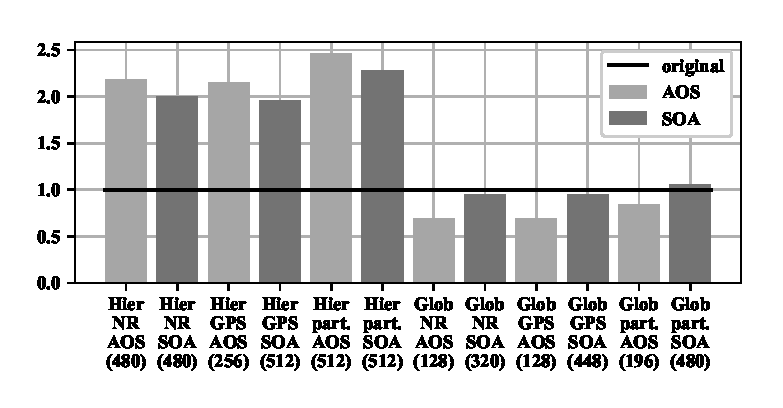
\includegraphics[width=9cm]{fig/volna_speedup.eps}
  \caption{\textbf{SpaceDiscretization} kernel speedup compared to the original
  code, done on a mesh with $3589735$ edges. The block sizes are shown in
  parentheses, the reordering algorithms are: the original reordering (NR), GPS
  reordering and partitioning (part.)}
  \label{fig:volna_speedup}
\end{figure}

On Volta, the performance of the kernel was $462$ GB/s ($62\%$ of the peak
bandwidth). Which means $1.18\times$ speedup on the kernel and $1.05\times$ 
speedup on the whole application compared to the original.



\subsubsection{Analysis of BookLeaf}

The measurements on the BookLeaf application (specifically the
\textbf{getacc\_scatter} kernel), as can be seen on Figures
\ref{fig:bookleaf_bw-vs-bs_hier} and \ref{fig:bookleaf_speedup}, also benefits
from the partitioning of the mesh.

The register count and occupancy are also similar to those with Airfoil ($64$
registers, achieving occupancy or around $40\%$), this leads to the variations
in performance along different block sizes.

With partitioning, the number of thread colours increased from $2$ to $5$, this
leads to the increased stalls from synchronisation: from $9\%$ to $20\%$, while
the reuse factor increases (from $2$ to $3.5$), which is comparable to that of
Airfoil, this explains the smaller increase in performance (only $9\%$, compared
to the $19\%$ increase in Airfoil).

The higher data reuse leads to $14\%$ and $41\%$ decrease of the number of
global transactions, for reads and writes, respectively. This large difference
between reads and writes is also because, like \textbf{SpaceDiscretization},
\textbf{getacc\_scatter} does not read values indirectly.

The best performance we achieved with \textbf{getacc\_scatter} results in  about
$2\%$ performance increase regarding the whole application. The useful bandwidth
also increased and reached $83\%$ of the peak stream bandwidth of the P100 GPU.

%shared mem: 17KB, with metis: 10.8


% bookleaf counters {{{ %
% Block size: 320
% Hier:                                                NR/AOS      NR/SOA     GPS/AOS     GPS/SOA   METIS/AOS   METIS/SOA
%                              Achieved Occupancy    0.430394    0.419929    0.430497    0.419961    0.434595    0.433032
%     Shared Memory Load Transactions Per Request    3.981157    3.289180    3.965366    3.279328    4.223552    3.869437
%    Shared Memory Store Transactions Per Request    3.317178    3.317178    3.313537    3.313537    3.884143    3.884143
%                   Device Memory Read Throughput  354.55GB/s  353.91GB/s  354.64GB/s  352.30GB/s  333.45GB/s  328.41GB/s
%                  Device Memory Write Throughput  104.92GB/s  105.59GB/s  104.86GB/s  105.02GB/s  67.486GB/s  69.298GB/s
%                        Shared Memory Efficiency      54.61%      60.09%      54.33%      59.75%      37.76%      39.35%
%                       Warp Execution Efficiency      99.50%      99.12%      99.38%      99.01%      95.70%      95.28%
%                            L2 Read Transactions     6811876     6855391     6809336     6852296     2636900     2676226
%                           L2 Write Transactions     2008024     2219229     2005901     2215992      509685      596673
%            Global Load Transactions Per Request    7.363423    7.884146    7.371714    7.880355    9.882201   10.026395
%           Global Store Transactions Per Request   15.672195    8.453975   15.672568    8.451264   15.785150    8.920493
%                 Device Memory Read Transactions     6792176     6810370     6789733     6807831     2588640     2616027
%                Device Memory Write Transactions     2010086     2031941     2007509     2029457      523903      552014
%                      Unified Cache Transactions     9270000     9153125     9267322     9150760     3651066     3644682
%           Issue Stall Reasons (Synchronization)       8.82%       9.02%       9.07%       9.45%      19.93%      20.05%
%              Issue Stall Reasons (Data Request)      74.74%      73.59%      74.26%      72.17%      58.52%      56.93%
%      Issue Stall Reasons (Execution Dependency)       6.73%       6.15%       6.76%       6.72%       8.03%       7.65%
%                                      Issued IPC    0.416526    0.360275    0.417040    0.395814    0.450024    0.424922
%                                     Issue Slots    14139389    13392697    14172617    13426925     6012129     5873760
%                          Issue Slot Utilization      18.71%      15.94%      18.72%      17.51%      20.02%      18.78%
%                 Eligible Warps Per Active Cycle    0.640313    0.549370    0.642497    0.608124    0.682836    0.655757
%                               Branch Efficiency      99.68%      99.66%      99.68%      99.66%      99.72%      99.68%
%        Warp Non-Predicated Execution Efficiency      96.92%      96.44%      96.81%      96.33%      93.02%      92.55%
%                    FLOP Efficiency(Peak Single)       0.00%       0.00%       0.00%       0.00%       0.00%       0.00%
%                    FLOP Efficiency(Peak Double)       1.63%       1.47%       1.62%       1.61%       1.63%       1.56%
%                   L2 Throughput (Texture Reads)  355.56GB/s  356.23GB/s  355.65GB/s  354.56GB/s  339.58GB/s  335.89GB/s
%                                    Executed IPC    0.416240    0.359758    0.416665    0.395579    0.452258    0.424822
%                         Multiprocessor Activity      98.40%      98.68%      98.39%      98.64%      95.56%      95.75%
%                         Number of Block Colours           4           4           4           4           9           9
%                                    Reuse Factor           2           2           2           2         3.5         3.5
%                       Average Cache Lines/Block         643         648         642         648         367         390
%                        Number of Thread Colours           2           2         2.1         2.1           5           5
%                                       Bandwidth     377GB/s     375GB/s     377GB/s     374GB/s     412GB/s     401GB/s
% }}} bookleaf counters %

\begin{figure}[Htbp]
  \centering
  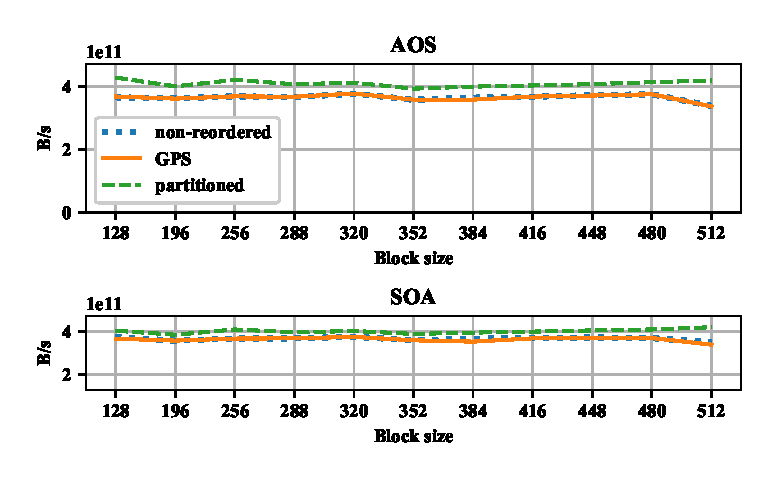
\includegraphics[width=9cm]{fig/bookleaf_bw-vs-bs_hier.eps}
  \caption{\textbf{getacc\_scatter} kernel bandwidth on a mesh with $4000000$
  edges using hierarchical colouring. Note that the y-axis doesn't start at the
  origin.}
  \label{fig:bookleaf_bw-vs-bs_hier}
\end{figure}

\begin{figure}[Htbp]
  \centering
  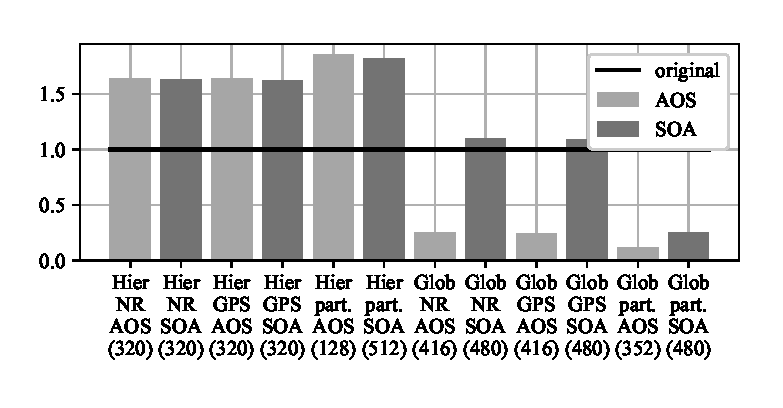
\includegraphics[width=9cm]{fig/bookleaf_speedup.eps}
  \caption{\textbf{getacc\_scatter} kernel speedup compared to the original
  code, done on a mesh with $4000000$ edges. The block sizes are shown in
  parentheses, the reordering algorithms are: the original reordering (NR), GPS
  reordering and partitioning (part.)}
  \label{fig:bookleaf_speedup}
\end{figure}

On Volta, the performance of the kernel was $631$ GB/s ($85\%$ of the peak
bandwidth which results in $1.03\times$ speedup on the whole application compared
to the original.


\subsubsection{Analysis of LULESH}\label{sec:analysis-of-lulesh}


The \textbf{IntegrateStressForElems} kernel uses a mapping with 8 neighbours
(compared to the 2--4 as in the case of the previous ones) for the brick
elements. Due to this, the number of colours is quite high: $8$, $16$ and $24$
in the global coloring versions (for the different reorderings), and $4$, $50$
and $15$ in the hierarchical colouring versions. The number of thread colours
was also quite high: $4$ in the non-reordered ($4.5$ in the GPS) and $11.6$ in
the partitioned version: this is a much higher increase compared to the previous
applications (Table \ref{tab:lulesh_counters_hier}). At the same time of course,
data reuse is higher compared to 2D applications - between $2.6$ and $4.8$.

The other aspect in which LULESH is different is that it uses a high amount of
registers ($96$), significantly decreases occupancy: with block size 320, the
AoS version achieved $15\%$ and the SoA version achieved around $30\%$.

Because of these two reasons, the synchronisation overhead ($39\%$ stalls were
from synchronisation on the partitioned mesh) couldn't be hidden: there were no
warps from other blocks to be scheduled in place of the stalled ones because
there was only one block running on each multiprocessor. The difference in
achieved occupancy also means that the SoA version with two blocks per
multiprocessor performs better.

\begin{figure}[Htbp]
  \centering
  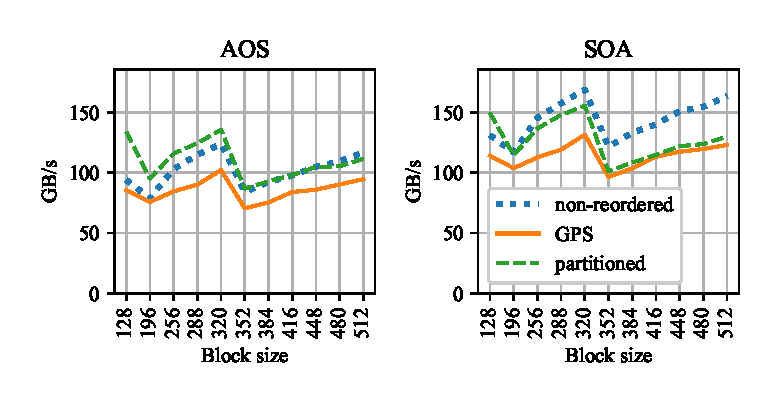
\includegraphics[width=9cm]{fig/lulesh_bw-vs-bs_hier.eps}
  \caption{\textbf{IntegrateStressForElems} kernel bandwidth on a mesh with
  $4913000$ cells using hierarchical colouring. Note that the y-axis doesn't
  start at the origin.}
  \label{fig:lulesh_bw-vs-bs_hier}
\end{figure}

Nevertheless, as shown on Figure \ref{fig:lulesh_speedup}, our hierarchical
colouring algorithm performs significantly better than the original, two-step
implementation, and also uses much less memory. Although the original needs less
synchronisation, the resulting warp divergence also cannot be hidden if the
occupancy is this low.

In the original version $37\%$ of the total time is spent in
\textbf{IntagrateStressForElems}, therefore the achieved $1.75\times$ speedup on
the kernel causes about $1.28\times$ speedup on the whole application. The
useful bandwidth in case of the best version of \textbf{IntegrateStressForElems}
reached $20\%$ of the peak stream bandwidth of the P100 GPU.

% lulesh counters {{{ %
% Block size: 320
% Hier:
%                                                      NR/AOS      NR/SOA     GPS/AOS     GPS/SOA   METIS/AOS   METIS/SOA
%                              Achieved Occupancy    0.153342    0.293920    0.153550    0.284203    0.153820    0.299256
%     Shared Memory Load Transactions Per Request    3.813638    3.526038    4.002716    3.631602    4.479968    4.322711
%    Shared Memory Store Transactions Per Request    3.316784    2.944442    3.508397    3.034623    3.742974    3.536361
%                   Device Memory Read Throughput  117.78GB/s  276.24GB/s  100.31GB/s  214.79GB/s  74.064GB/s  155.87GB/s
%                  Device Memory Write Throughput  44.459GB/s  99.108GB/s  38.989GB/s  79.804GB/s  26.038GB/s  54.191GB/s
%                        Shared Memory Efficiency      48.54%      53.36%      45.44%      50.98%      30.47%      31.81%
%                       Warp Execution Efficiency      97.64%      96.94%      97.39%      96.41%      91.39%      89.82%
%                            L2 Read Transactions     8927298     8925744      733415      739319     1621952     1715366
%                    L2 Read Transactions (total)    35709192    35702976    36670750    36965950    24329280    25730490
%                           L2 Write Transactions     3429290     3433123      281319      288606      574252      631224
%                   L2 Write Transactions (total)    13717160    13732492    14065950    14430300     8613780     9468360
%            Global Load Transactions Per Request    8.461524    9.445318    8.365310    9.635046    8.782532    9.537800
%           Global Store Transactions Per Request    8.659927    8.668800    8.650857    8.798241    9.222445   10.001870
%                 Device Memory Read Transactions     8393075     8851961      690624      727464     1525893     1668476
%         Device Memory Read Transactions (total)    33572300    35407844    34531200    36373200    22888395    25027140
%                Device Memory Write Transactions     3168271     3175906      268437      270294      536445      580062
%        Device Memory Write Transactions (total)    12673084    12703624    13421850    13514700     8046675     8700930
%                      Unified Cache Transactions    12854357    11281423     1048169      918060     2389410     2202778
%              Unified Cache Transactions (total)    51417428    45125692    52408450    45903000    35841150    33041670
%           Issue Stall Reasons (Synchronization)      13.27%      19.06%      14.11%      17.78%      39.46%      41.75%
%              Issue Stall Reasons (Data Request)      63.80%      56.40%      61.52%      55.14%      34.65%      30.51%
%      Issue Stall Reasons (Execution Dependency)      12.35%      10.16%      12.52%      10.18%      14.20%      12.85%
%                                    Executed IPC    0.316365    0.514800    0.319681    0.472282    0.295742    0.488715
%                                      Issued IPC    0.316544    0.513558    0.320049    0.473822    0.295894    0.490463
%                                     Issue Slots    46704488    32475988     3815312     2649675    11050475     9059009
%                             Issue Slots (total)   186817952   129903952   190765600   132483750   165757125   135885135
%                          Issue Slot Utilization      15.03%      23.13%      15.19%      21.32%      13.79%      22.20%
%                         Multiprocessor Activity      98.82%      98.50%      89.85%      90.13%      96.44%      94.58%
%                 Eligible Warps Per Active Cycle    0.587770    1.128024    0.588915    1.037127    0.550260    1.021502
%                               Branch Efficiency      99.36%      99.12%      99.42%      99.21%      99.41%      99.32%
%        Warp Non-Predicated Execution Efficiency      96.62%      95.45%      96.40%      94.95%      90.27%      88.38%
%                    FLOP Efficiency(Peak Single)       0.00%       0.00%       0.00%       0.00%       0.00%       0.00%
%                    FLOP Efficiency(Peak Double)       5.16%      11.43%       4.65%       9.42%       5.16%       9.91%
%                   L2 Throughput (Texture Reads)  125.25GB/s  278.49GB/s  106.33GB/s  217.85GB/s  78.652GB/s  160.10GB/s
%                         Number of Block Colours           4           4          50          50          15          15
%                                    Reuse Factor         2.6         2.6         2.5         2.5         4.8         4.8
%                       Average Cache Lines/Block         744         747         770         781         427         474
%                        Number of Thread Colours           4           4         4.5         4.5        11.6        11.6
%                                       Bandwidth     124GB/s     168GB/s     102GB/s      94GB/s     129GB/s     147GB/s
% }}} lulesh counters %

\begin{figure}[Htbp]
  \centering
  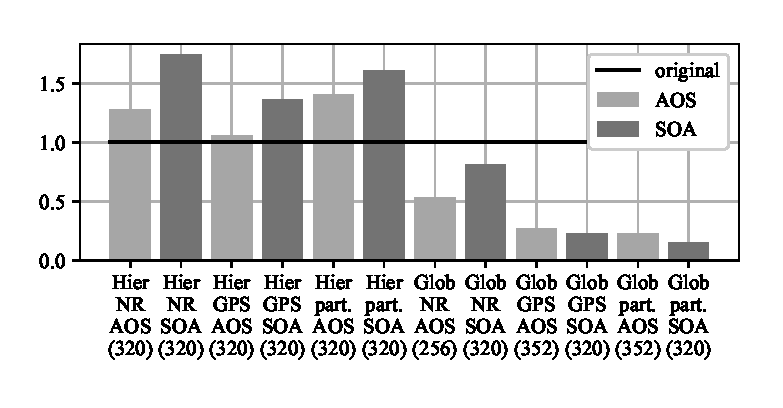
\includegraphics[width=9cm]{fig/lulesh_speedup.eps}
  \caption{\textbf{IntegrateStressForElems} kernel speedup compared to the
  original (gathering) code, done on a mesh with $4913000$ cells. The block
  sizes are shown in parentheses, the reordering algorithms are: the original
  reordering (NR), GPS reordering and partitioning (part.)}
  \label{fig:lulesh_speedup}
\end{figure}

\begin{table}[Htbp]
  \centering
  \resizebox{\columnwidth}{!}{
  % \begin{tabular}{|R{2.5cm}|cc|c|c|}
    \small
  \begin{tabular}{|r|cc|c|c||c|}
    \hline
      Reordering  & \multicolumn{2}{c|}{none} & \multicolumn{2}{c||}{partition} & original\\
      \hline
      Data layout &    AOS      &   SOA     &     AOS      &    SOA & SOA\\
      \hline
                               Bandwidth (GB/s) &   $ 124$ &   $ 168$ &   $ 129$ &   $ 147$ & $97$\\
                               Runtime (ms)     &   $5.45$ & $4.00$ & $4.98$ & $4.34$ & $6.98$ \\
                             Achieved Occupancy &   $0.15$ &   $0.29$ &   $0.15$ &   $0.30$ & $0.24$\\
        Global Memory Read Transactions (total) &   \num{33572}k & \num{35408}k &   \num{22888}k &   \num{25027}k  & \num{16072}k\\
       Global Memory Write Transactions (total) &   \num{12673}k & \num{12704}k &   \num{ 8047}k &   \num{ 8701}k  & \num{32689}k\\
                        Number of Block Colours &   $       4$ &   $       4$ & $      15$ &   $      15$ & - \\
                       Number of Thread Colours &   $       4$ &   $       4$ & $    11.6$ &   $    11.6$  & -\\
                                   Reuse Factor &   $     2.6$ &   $     2.6$ & $     4.8$ &   $     4.8$ & -\\
          Issue Stall Reasons (Synchronization) &   $  13\%$ &   $  19\%$ &   $ 39\%$ &   $  42\%$  & $0\%$\\
             Issue Stall Reasons (Data Request) &   $  64\%$ &   $  56\%$ &   $ 35\%$ &   $  31\%$  & $26\%$\\
                      Average Cache Lines/Block &   $     744$ &   $     747$ & $     427$ &   $     474$  & -\\
                      Warp Execution Efficiency &   $  98\%$ &   $  97\%$ &   $ 91\%$ &   $  90\%$ & $100\%$\\
      \hline
      Block size & \multicolumn{4}{c||}{$320$} & $64$\\

    \hline
  \end{tabular}
  }
  \caption{Collected performance metrics of the hierarchical colouring
    implementation of the \textbf{IntegrateStressForElems} kernel. The last
    column is the measured performance of the original code.}
  \label{tab:lulesh_counters_hier}
\end{table}

% TODO reformulate this paragraph
On Volta, we achieved $1.84\times$ speedup in the kernel compared to the
original code with $273$ GB/s bandwidth ($37\%$ of the peak bandwidth). In the
original version $35\%$ of the total time is spent in
\textbf{IntegrateStressForElems}, therefore the achieved kernel speedup causes
about $1.29\times$ speedup on the whole application.

\subsubsection{Analysis of miniAero}

The \textbf{compute\_face\_flux} kernel is the most computationally intensive
among the ones we tested: it uses $165$ registers in hierarchical  colouring
($166$ in SoA layout). Also, it achieves (with block size $384$ and reordered by
GPS) $15\%$ of peak double precision efficiency, compared to the $6$--$7\%$ in
Airfoil (Table \ref{tab:mini_aero_counters_hier}). It also uses $8$ square root
operations and several divides that can't efficiently fill the pipelines at such
low occupancy.

The amount of data indirectly accessed by the kernel is also large: each thread
accesses $2$ data points indirectly, each holding $32$ double precision values.
If all of that is loaded into shared memory, the size of it exceeds the hardware
limits with block sizes larger than $288$; it didn't run with the original mesh
numbering with any block size, and only with smaller block sizes on the reordered meshes (Figure \ref{fig:mini_aero_bw_crash}). The other measurements were carried out
by only loading the incremented data into shared memory.

\begin{figure}[Htbp]
  \centering
  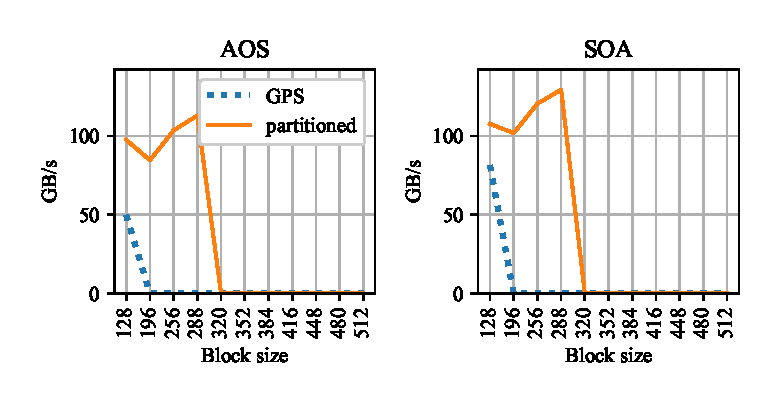
\includegraphics[width=9cm]{fig/mini_aero_bw_crash.eps}
  \caption{The \textbf{compute\_face\_flux} kernel bandwidth on a mesh with
  $6242304$ faces. The kernel didn't run in the cases where the data reuse was
  not high enough because the large amount of shared memory needed; these are
  shown here with $0$ bandwidth.}
  \label{fig:mini_aero_bw_crash}
\end{figure}

The mesh also has a complex structure ($18$ and $15$ block colours for GPS
reordered and partitioned versions, respectively) and the original ordering was
far from optimal: we couldn't run the non-reordered version, because the number
of block colours exceeded the implementation limit of the library, which is
$256$.

As with LULESH, only one block was running at a time on each multiprocessor.
Although the synchronisation overhead was lower ($3$ and $6$ thread
colours in the GPS reordered and partitioned versions, respectively), the costly
operations prevented high performance gains in the case of the partitioned
version (Figure \ref{fig:mini_aero_bw_small-cache}).

\begin{figure}[Htbp]
  \centering
  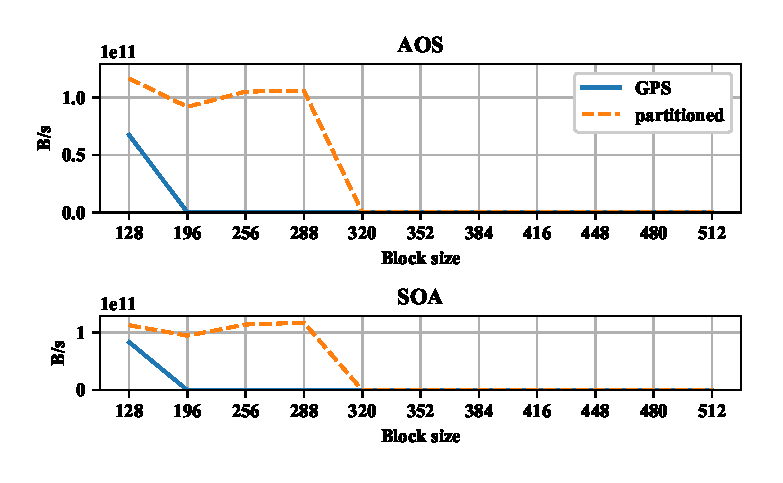
\includegraphics[width=9cm]{fig/mini_aero_bw_small-cache.eps}
  \caption{The \textbf{compute\_face\_flux} kernel bandwidth on a mesh with
  $6242304$ faces. The shared memory was only used to cache the increments,
  reducing the need for large shared memory size. The kernel didn't fit into the
  shared memory with block size larger than $384$ or if not reordered because
  the large amount of shared memory needed; these are shown here with $0$
  bandwidth.}
  \label{fig:mini_aero_bw_small-cache}
\end{figure}

The original Kokkos implementation either used atomic adds or the two-step
gathering approach depending on compilation parameters. Our implementation
outperformed both (Figure \ref{fig:mini_aero_speedup_small-cache}), for the same
reason as in case of LULESH.

In the original version $22\%$ of the total time is spent in
\textbf{compute\_face\_flux}, therefore the achieved $1.75\times$ kernel speedup
causes about $1.10\times$ speedup on the whole application. The useful bandwidth
in case of the best version of \textbf{compute\_face\_flux} ($168$ GB/s) reached
$34\%$ of the peak stream bandwidth of the P100 GPU.

% mini_aero counters {{{ %
% Block size: 128
% Hier:                                            GPS/AOS        GPS/SOA   METIS/AOS   METIS/SOA
%                              Achieved Occupancy    0.061617    0.060943    0.121864    0.121086
%     Shared Memory Load Transactions Per Request    3.089353    2.930011    4.559967    4.435671
%    Shared Memory Store Transactions Per Request    4.597106    2.132409    4.931486    2.612757
%                   Device Memory Read Throughput  84.899GB/s  154.47GB/s  113.68GB/s  185.10GB/s
%                  Device Memory Write Throughput  10.564GB/s  19.753GB/s  14.249GB/s  21.629GB/s
%                        Shared Memory Efficiency      49.82%      66.99%      33.81%      40.56%
%                       Warp Execution Efficiency      91.41%      84.43%      88.06%      85.42%
%                            L2 Read Transactions     3746994     4192153     3322917     4813039
%                    L2 Read Transactions (total)    74939880    83843060    56489589    81821663
%                           L2 Write Transactions      450646      544462      374918      576190
%                   L2 Write Transactions (total)     9012920    10889240     6373606     9795230
%            Global Load Transactions Per Request    8.363060    9.608935    9.101123   11.272758
%           Global Store Transactions Per Request    8.928965    8.552480   10.217068   13.250228
%                 Device Memory Read Transactions     3678059     4101386     3141355     4534744
%         Device Memory Read Transactions (total)    73561180    82027720    53403035    77090648
%                Device Memory Write Transactions      457662      524480      393745      529889
%        Device Memory Write Transactions (total)     9153240    10489600     6693665     9008113
%                      Unified Cache Transactions     5026525     4529910     4429316     4059892
%              Unified Cache Transactions (total)   100530500    90598200    75298372    69018164
%           Issue Stall Reasons (Synchronization)       4.33%       8.66%      15.13%      20.92%
%              Issue Stall Reasons (Data Request)      60.60%      35.22%      47.30%      34.50%
%      Issue Stall Reasons (Execution Dependency)      23.06%      32.73%      22.71%      23.30%
%                                    Executed IPC    0.252724    0.375217    0.472362    0.496491
%                                      Issued IPC    0.253601    0.375074    0.472305    0.496602
%                                     Issue Slots    22380958    19376361    23994392    21907800
%                             Issue Slots (total)   447619160   387527220   407904664   372432600
%                          Issue Slot Utilization      11.90%      16.92%      21.96%      22.51%                                                 
%                         Multiprocessor Activity      98.16%      97.83%      98.53%      98.68% 
%                 Eligible Warps Per Active Cycle    0.265263    0.383198    0.534554    0.552878
%                               Branch Efficiency      99.45%      99.42%      99.42%      99.31%
%        Warp Non-Predicated Execution Efficiency      90.54%      83.43%      87.06%      84.18%
%                    FLOP Efficiency(Peak Double)       4.95%       8.38%       9.77%      11.50%
%                   L2 Throughput (Texture Reads)  86.394GB/s  157.71GB/s  120.09GB/s  196.28GB/s
%                         Number of Block Colours         20          20          17          17
%                                    Reuse Factor       1.98        1.98        3.26        3.26
%                       Average Cache Lines/Block        169         189         116         179
%                        Number of Thread Colours          3           3           6           6
%                                       Bandwidth
% }}} mini_aero counters %

\begin{figure}[Htbp]
  \centering
  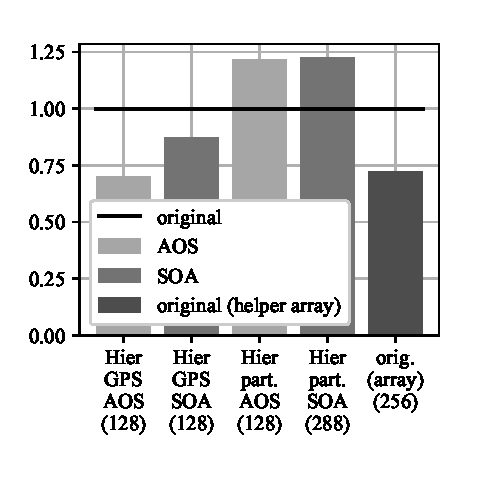
\includegraphics[width=9cm]{fig/mini_aero_speedup_nocache.eps}
  \caption{The \textbf{compute\_face\_flux} kernel speedup compared to the
  original code that was using atomic adds, on a mesh with
  $6242304$ faces. The shared memory was only used to cache the increments,
  reducing the need for large shared memory size. The last bar shows the
  relative performance of the original code with the helper array approach.}
  \label{fig:mini_aero_speedup_small-cache}
\end{figure}

\begin{table}[Htbp]
  \centering
  \resizebox{\columnwidth}{!}{
    \small
  % \begin{tabular}{|R{2.5cm}|cc|c|c|}
  \begin{tabular}{|r|cc|c|c||c|}
    \hline
      Reordering  & \multicolumn{2}{c|}{GPS} & \multicolumn{2}{c||}{partition} & original\\
      \hline
      Data layout &    AOS      &   SOA     &     AOS      &    SOA & SOA\\
      \hline
                               Bandwidth (GB/s)&    $  67$ &   $ 84$ &   $ 117$ &   $ 113$ & $96$\\
                               Runtime (ms)    &    $19.09$ & $15.38$ & $11.04$
                               & $11.38$ & $13.39$\\
                             Achieved Occupancy&    $0.06$ & $0.06$ & $0.12$ & $0.12$  & $0.23$\\
                Global Memory Read Transactions&    $73561\text{k}$ & $82028\text{k}$ & $53403\text{k}$ & $77091\text{k}$  & $87368\text{k}$\\
               Global Memory Write Transactions&    $9153\text{k}$ & $10390\text{k}$ & $6694\text{k}$ & $9008\text{k}$ & $5934\text{k}$ \\
                        Number of Block Colours&    $      18$ &   $      18$ & $      15$ &   $      15$  & -\\
                       Number of Thread Colours&    $       3$ &   $       3$ & $       6$ &   $       6$  & -\\
                                   Reuse Factor&    $     2.2$ &   $     2.2$ & $     3.9$ &   $     3.9$  & -\\
          Issue Stall Reasons (Synchronization)&    $4\%$ & $9\%$ & $15\%$ & $21\%$    & $0\%$ \\
             Issue Stall Reasons (Data Request)&    $61\%$ & $35\%$ & $47\%$ & $35\%$  & $49\%$\\
     Issue Stall Reasons (Execution Dependency)&    $23\%$ & $33\%$ & $23\%$ & $23\%$  & $13\%$\\
                      Average Cache Lines/Block&    $     452$ &   $     471$ & $     269$ &   $     344$  & -\\
                      Warp Execution Efficiency&    $91\%$ & $84\%$ & $88\%$ & $85\%$  & $91\%$\\
                   FLOP Efficiency(Peak Double)&    $5\%$ & $8\%$ & $10\%$ & $12\%$  & $8\%$\\
      \hline
      Block size & \multicolumn{4}{c||}{128} & 256\\
    \hline
  \end{tabular}
  }
  \caption{Collected performance metrics of the hierarchical colouring
    implementation of the \textbf{compute\_face\_flux} kernel. The last column
    is the measured performance of the original code.}
  \label{tab:mini_aero_counters_hier}
\end{table}

% TODO reformulate this paragraph
On Volta, we achieved $2.57\times$ speedup in the kernel compared to the
original code with $268$ GB/s bandwidth ($36\%$ of the peak bandwidth). In the
original version $27\%$ of the total time is spent in
\textbf{compute\_face\_flux}, therefore the kernel speedup causes about
$1.20\times$ speedup on the whole application.


\subsubsection{Analysis of structured meshes}

As mentioned in Sections \ref{sec:mini-aero-summary} and
\ref{sec:lulesh-summary}, the meshes of miniAero and LULESH are actually structured meshes, generated by the
code itself. This lets us to use the structured nature of the mesh to create partitions with netter shapes than what METIS produces. This in turn allows us to understand the trade-off between
high data reuse and few thread colours used more by creating 1D, 2D and 3D
partitions (these will have an increasing amount of reuse and number of colours).

While both kernels operate on 3D Cartesian (hex8) meshes, the
\textbf{IntegrateStressForElems} kernel in LULESH uses a mapping from cells to their
connected vertices, and the \textbf{compute\_face\_flux} kernel in miniAero maps from
(internal) faces to cells. We then created a number of different partition shapes - 1D lines, 2D rectangles and 3D bricks.

%In the former case, the blocks are created from the
%cells as rectangles.
% In the second case, the creation starts the same way, but at the last axis (the
% contiguous axis) three faces corresponding to one cell are added to the block at
% the same time. This way the blocks cover the whole mesh similarly to the
% previous case. This also means that when the block is long along the third axis,
% the reuse will be higher than it would be with the other two axes. Because of
% this, in our measurements, we ordered the dimensions of the blocks so that they
% are longest along this axis.

Figures \ref{fig:lulesh_block} and \ref{fig:mini_aero_block} show the
bandwidths, reuse factors and the number of thread colours across different
block-shapes, along with the result of partitioning the same mesh using METIS.
The size of the blocks is $128$. These measurements were run on meshes with
shape specifically tailored so that the handcrafted blocks can cover them
without any gaps.

In \textbf{IntegrateStressForElems}, the bandwidth of the original ordering achieved  $134\,\text{GB/s}$ - it uses a row major order, similar to ours
when we use a block shape that is $128$ cells long and only $1$ cell thin in the
other dimensions. The partitioned mesh (detailed
in Section \ref{sec:analysis-of-lulesh}) achieved $132\,\text{GB/s}$, and we achieved $167\,\text{GB/s}$
bandwidth using our handcrafted blocks, for the same block size ($128$). Note
that using regular shapes is better for the thread colouring algorithm too: with
METIS partitioning, the number of colours needed is higher than in the other
cases.

For \textbf{compute\_face\_flux}, we achieved $167\,\text{GB/s}$ bandwidth,
compared to $101\,\text{GB/s}$ achieved with METIS partitioning.

Of course, using these handcrafted blocks can only be done on meshes that are actually structured, therefore this is not representative of realistic cases. However, these results illustrate clearly that when
the number of thread colours are the same, increased reuse leads to better
performance. Also, there is an optimal number of thread colours for each
application, and performance will suffer above that. The challenge lies in
finding a partitioning algorithm that can either find the middle ground, or can
be tuned along the amount of reuse it aims to achieve. Such partitioning algorithms are not currently available, but we demonstrate a clear need for them.

\begin{figure}[Htbp]
  \centering
  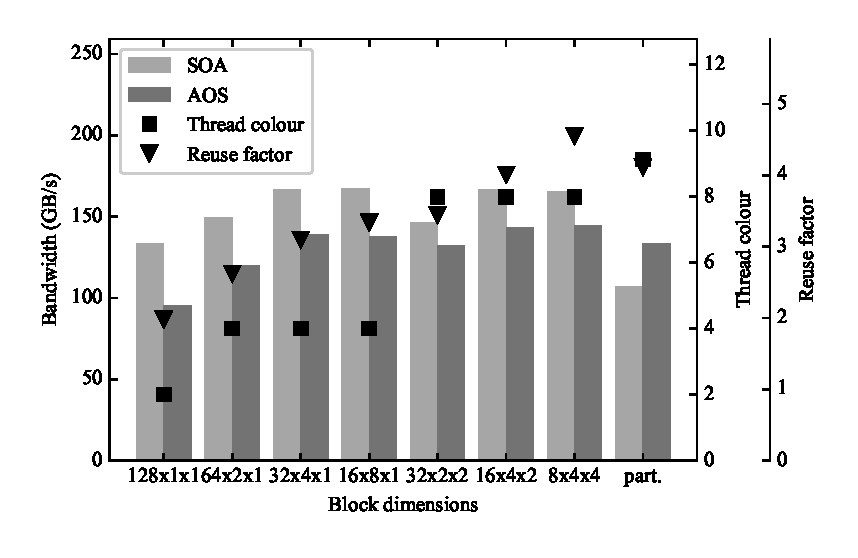
\includegraphics[width=12cm]{fig/lulesh_block.eps}
  \caption{\textbf{IntegrateStressForElems} kernel with explicitly controlled
  partitioning. For comparison, the last column shows the result on the same
  mesh, partitioned by METIS.}
  \label{fig:lulesh_block}
\end{figure}

\begin{figure}[Htbp]
  \centering
  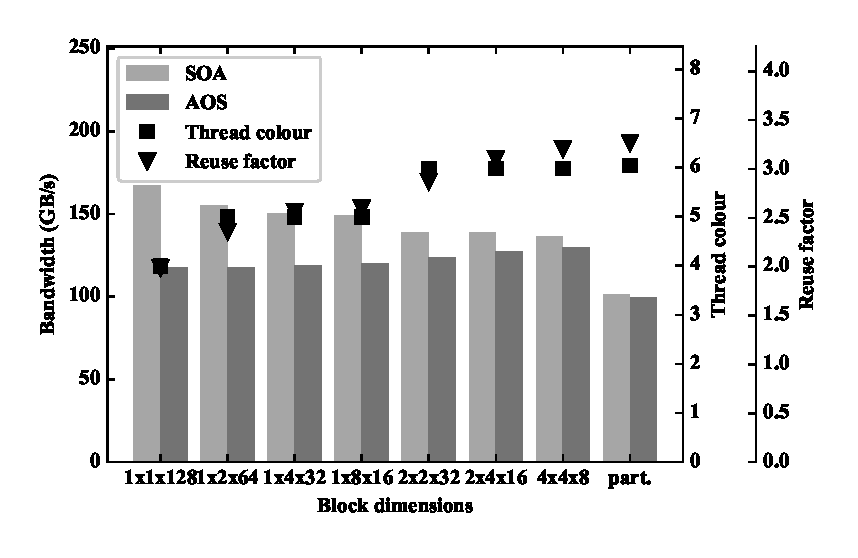
\includegraphics[width=12cm]{fig/mini_aero_block.eps}
  \caption{\textbf{compute\_face\_flux} kernel with explicitly controlled
  partitioning. For comparison, the last column shows the result on the same
  mesh, partitioned by METIS.}
  \label{fig:mini_aero_block}
\end{figure}

% vim:set et sw=2 ts=2 tw=80 fdm=marker:
